\documentclass[11pt]{article}
\usepackage[spanish]{babel}
\usepackage[utf8]{inputenc}
\usepackage{amsmath}
\usepackage{geometry}
\usepackage{graphicx}
\usepackage{listings}
\usepackage{xcolor}
\graphicspath{{../images/}}
\geometry{margin=2.5cm}

\definecolor{matlabkeyword}{rgb}{0,0,1}
\definecolor{matlabcomment}{rgb}{0.13,0.55,0.13}
\definecolor{matlabstring}{rgb}{0.63,0.13,0.94}
\definecolor{matlabbg}{rgb}{0.97,0.97,0.97}

\lstdefinelanguage{Matlab}{
  keywords={break,case,catch,continue,else,elseif,end,for,function,global,if,otherwise,persistent,return,switch,try,while},
  keywordstyle=\color{matlabkeyword}\bfseries,
  sensitive=true,
  comment=[l]{\%},
  commentstyle=\color{matlabcomment}\itshape,
  string=[b]',
  stringstyle=\color{matlabstring},
  morestring=[b]"
}

\lstset{
  language=Matlab,
  backgroundcolor=\color{matlabbg},
  basicstyle=\ttfamily\small,
  breaklines=true,
  columns=fullflexible,
  frame=single,
  numbers=left,
  numberstyle=\tiny\color{gray},
  showstringspaces=false
}

\title{Taller potencia --- Ejercicio 4}
\author{}
\date{}

\begin{document}
\maketitle

\section*{Enunciado}

\textit{4. El rectificador controlado de la figura 4, se alimenta con
Vs=30(b+c)V, f=60Hz; si R=(a+b+c)$\Omega$; L=60mH y $\alpha=45^\circ$;
determinar: a) los tiempos $t_1$ y $t_e$, el \'angulo de extinci\'on para la
se\~nal de entrada y el tipo de corriente que corresponde, dibuje las se\~nales
de $v_o$ e $i_o$, b) Las corrientes y tensiones dc y rms, las potencias
activa y aparente, el factor de potencia, la eficiencia y los factores de
rizo.}

\begin{figure}[h]
\centering
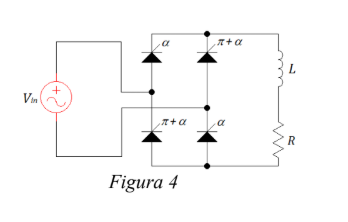
\includegraphics[width=0.6\textwidth]{circuito_rectificador_puente_controlado_figura4.png}
\caption{Rectificador controlado de la figura 4 (puente completo, $\alpha$ y $\pi+\alpha$).}
\end{figure}

\section*{Datos}

\begin{align*}
a &= 3,\quad b = 9,\quad c = 3 \\
V_s &= 30(9+3) = 360\ \text{V} \\
f &= 60\ \text{Hz} \\
R &= (3+9+3)\ \Omega = 15\ \Omega \\
L &= 60\ \text{mH} \\
\alpha &= 45^\circ = 0{,}7854\ \text{rad}
\end{align*}

\section*{Constante de tiempo y $t_1$}

\begin{align*}
\tau &= \frac{60\times10^{-3}}{15\ \Omega} = 0{,}004\ \text{s} \\
\frac{1}{\tau} &= 250\ \text{s}^{-1} \\
\omega &= 2\pi(60\ \text{Hz}) = 376{,}991\ \text{rad/s} \\
t_1 &= \frac{0{,}7854}{376{,}991} = \boxed{2{,}0833\ \text{ms}}
\end{align*}

\section*{Impedancia}

\begin{align*}
Z &= 15\ \Omega + j(120\pi)(60\times10^{-3}) = 15\ \Omega + j22{,}6195 \\
|Z| &= \sqrt{(22{,}6195)^2+(15)^2} = 27{,}14\ \Omega \\
\varphi &= \tan^{-1}\!\left(\frac{22{,}6195}{15}\right) = 0{,}9852\ \text{rad} \\
Z &= 27{,}14\ \Omega \angle 0{,}9852
\end{align*}

\section*{Corriente forzada}

\begin{align*}
V_m &= 360\ \text{V}\cdot\sqrt{2} = 509{,}12\ \text{V} \\
I_f &= \frac{509{,}12\ \text{V}\angle 0}{27{,}14\ \Omega\angle 0{,}9852} = 18{,}76\ \text{A}\angle{-0{,}9852}
\end{align*}

\begin{align*}
i(t) = 18{,}76\,\sen(120\pi t - 0{,}9852) + I_o\,e^{-250(t-0{,}0020833)}
\end{align*}

\section*{Condici\'on inicial ($i(t_1)=0$)}

\begin{align*}
0 &= 18{,}76\,\sen(0{,}7854 - 0{,}9852) + I_o \\
0 &= 18{,}76\,(-0{,}1985) + I_o \\
0 &= -3{,}724 + I_o \\
I_o &= \boxed{3{,}724\ \text{A}}
\end{align*}

\section*{Verificaci\'on del tipo de corriente}

Se eval\'ua $i(t)$ en $t=(\pi+\alpha)/\omega$ (instante del siguiente disparo):

\begin{align*}
\frac{\pi+\alpha}{\omega} &= \frac{3{,}9270}{376{,}991} = 10{,}419\ \text{ms} \\
i(10{,}419\ \text{ms}) &= 18{,}76\,\sen(2{,}9418) + 3{,}724\,e^{-250(0{,}010419-0{,}0020833)} \\
&= 18{,}76\,(0{,}1985) + 3{,}724\,(0{,}1244) = 3{,}724 + 0{,}4634 = \boxed{4{,}187\ \text{A}}
\end{align*}

Como $i(\pi+\alpha) = 4{,}187$~A $>0$, la corriente \textbf{no llega a cero}
antes del siguiente disparo $\Rightarrow$ \textbf{la corriente es continua}
(por lo tanto no existe $t_e$ ni \'angulo de extinci\'on: la conducci\'on es
ininterrumpida y se traslapa con el disparo siguiente).

\section*{Corrientes y tensiones DC y RMS (por serie de Fourier)}

\paragraph{Definici\'on de la se\~nal (de $-T/2$ a $T/2$, con $T=2\pi/\omega$):}
\begin{align*}
v_o(\theta) = V_m\,\sen(\theta), \qquad \alpha \le \theta \le \pi+\alpha
\end{align*}
(se repite peri\'odicamente cada $\pi$ radianes; al ser continua, $v_o$ nunca
vale cero dentro del intervalo de conducci\'on, a diferencia del caso
discontinuo donde el tramo $[\beta,\pi+\alpha]$ es cero).

\paragraph{Planteamiento de las integrales (excepci\'on: en el rectificador
controlado se permite usar la forma cerrada tras plantear la integral):}
\begin{align*}
a_n &= \frac{1}{\pi}\int_{\alpha}^{\pi+\alpha} V_m\,\sen(\theta)\cos(n\theta)\,d\theta
     = \frac{2V_m}{\pi}\left[\frac{\cos((n+1)\alpha)}{n+1} - \frac{\cos((n-1)\alpha)}{n-1}\right] \\
b_n &= \frac{1}{\pi}\int_{\alpha}^{\pi+\alpha} V_m\,\sen(\theta)\sen(n\theta)\,d\theta
     = \frac{2V_m}{\pi}\left[\frac{\sen((n+1)\alpha)}{n+1} - \frac{\sen((n-1)\alpha)}{n-1}\right]
\end{align*}

\paragraph{Para n=0 (componente DC):}
\begin{align*}
V_{DC} &= \frac{1}{\pi}\int_{\alpha}^{\pi+\alpha} V_m\,\sen(\theta)\,d\theta = \frac{2V_m}{\pi}\cos(\alpha) = \frac{2(509{,}12)}{\pi}\cos(45^\circ)
        = 324{,}07\cdot 0{,}7071 = \boxed{229{,}2\ \text{V}} \\
I_{DC} &= \frac{229{,}2}{15} = \boxed{15{,}28\ \text{A}}
\end{align*}

\paragraph{Para n=2:}
\begin{align*}
Z_2 &= 15 + j240\pi(0{,}06) = 47{,}67\ \Omega\angle 1{,}251 \\
a_2 &= \frac{2(509{,}12)}{\pi}\left[\frac{\cos(3\cdot45^\circ)}{3} - \cos(45^\circ)\right] = 324{,}07(-0{,}9428) = -305{,}6\ \text{V} \\
b_2 &= \frac{2(509{,}12)}{\pi}\left[\frac{\sen(3\cdot45^\circ)}{3} - \sen(45^\circ)\right] = 324{,}07(-0{,}4714) = -152{,}8\ \text{V} \\
V_2 &= \sqrt{(-305{,}6)^2+(-152{,}8)^2} = 341{,}6\ \text{V} \\
I_2 &= \frac{341{,}6}{47{,}67} = 7{,}166\ \text{A}
\end{align*}

Los dem\'as arm\'onicos ($n=4,6,8,10,12,14$) se obtienen igual, cambiando
$(n+1)$ y $(n-1)$, con $Z_n=15+jn(120\pi)(0{,}06)$:

\begin{center}
\begin{tabular}{c c c c c c}
$n$ & $a_n$ (V) & $b_n$ (V) & $V_n$ (V) & $Z_n$ ($\Omega\angle$rad) & $I_n$ (A) \\ \hline
0 & --- & --- & 229{,}2 & 15 & $I_{DC}=15{,}28$ \\
2 & $-305{,}6$ & $-152{,}8$ & 341{,}6 & $47{,}67\angle1{,}251$ & 7{,}166 \\
4 & 30{,}6 & $-122{,}2$ & 126{,}0 & $91{,}71\angle1{,}406$ & 1{,}373 \\
6 & 78{,}6 & 13{,}1 & 79{,}6 & $136{,}6\angle1{,}461$ & 0{,}583 \\
8 & $-7{,}3$ & 58{,}2 & 58{,}7 & $181{,}6\angle1{,}489$ & 0{,}323 \\
10 & $-46{,}3$ & $-4{,}6$ & 46{,}5 & $226{,}7\angle1{,}505$ & 0{,}205 \\
12 & 3{,}2 & $-38{,}5$ & 38{,}6 & $271{,}9\angle1{,}516$ & 0{,}142 \\
14 & 32{,}9 & 2{,}4 & 33{,}0 & $317{,}0\angle1{,}523$ & 0{,}104 \\
\end{tabular}
\end{center}

\begin{align*}
V_{RMS} &= \sqrt{229{,}2^2 + \tfrac{1}{2}\left(341{,}6^2+126{,}0^2+79{,}6^2+58{,}7^2+46{,}5^2+38{,}6^2+33{,}0^2\right)} \\
        &= \boxed{355{,}0\ \text{V}}
\end{align*}

\begin{align*}
I_{RMS} &= \sqrt{15{,}28^2 + \tfrac{1}{2}\left(7{,}166^2+1{,}373^2+0{,}583^2+0{,}323^2+0{,}205^2+0{,}142^2+0{,}104^2\right)} \\
        &= \boxed{16{,}14\ \text{A}}
\end{align*}

\section*{Potencias}

\begin{align*}
P &= 16{,}14^2 \cdot 15 = \boxed{3905{,}7\ \text{W}} \\
P_{DC} &= 229{,}2 \cdot 15{,}28 = \boxed{3501{,}6\ \text{W}} \\
S &= 360 \cdot 16{,}14 = \boxed{5810{,}4\ \text{VA}}
\end{align*}

\section*{Factor de potencia y eficiencia}

\begin{align*}
FP &= \frac{3905{,}7}{5810{,}4} = \boxed{0{,}672} \\
\eta &= \frac{3501{,}6}{5810{,}4} = \boxed{0{,}603}
\end{align*}

\section*{Factores de rizo}

\begin{align*}
FR_V &= \frac{\sqrt{355{,}0^2 - 229{,}2^2}}{229{,}2} = \boxed{1{,}18} \\
FR_I &= \frac{\sqrt{16{,}14^2 - 15{,}28^2}}{15{,}28} = \boxed{0{,}339}
\end{align*}

\section*{An\'alisis y diagramas}

Como la corriente es continua, $v_o(t)$ sigue $V_m\sen(\omega t)$ de forma
ininterrumpida (con un salto en cada disparo, pero sin tramos en cero); $i_o(t)$
tampoco llega a cero salvo en el instante exacto del relevo entre pares de
tiristores. Las se\~nales se grafican en la ventana $[t_1,(\pi+\alpha)/\omega]$
(un periodo representativo), usando solo los comandos de MATLAB permitidos:

\begin{lstlisting}[language=Matlab, caption={C\'odigo MATLAB -- Ejercicio 4}, label={lst:ex4}]
x=linspace(0.0020833,0.010419,200);
vo=509.12*sin(376.991*x);
plot(x*1e3,vo,'b','LineWidth',1.5); hold on
title('Tension de salida vo(t)'); xlabel('Tiempo (ms)'); ylabel('Tension (V)')

x=linspace(0.0020833,0.010419,200);
io=18.76*sin(376.991*x-0.9852)+3.724*exp(-250*(x-0.0020833));
plot(x*1e3,io,'r','LineWidth',1.5); hold on
title('Corriente de salida io(t)'); xlabel('Tiempo (ms)'); ylabel('Corriente (A)')
\end{lstlisting}

\begin{figure}[h]
\centering
\includegraphics[width=0.75\textwidth]{ejercicio4_tension_salida_vo_alpha45.png}
\caption{Tensi\'on de salida $v_o(t)$ -- Ejercicio 4 ($\alpha=45^\circ$, corriente continua).}
\end{figure}

\begin{figure}[h]
\centering
\includegraphics[width=0.75\textwidth]{ejercicio4_corriente_salida_io_alpha45.png}
\caption{Corriente de salida $i_o(t)$ -- Ejercicio 4 ($\alpha=45^\circ$, corriente continua).}
\end{figure}

\end{document}
